\documentclass[10pt]{article}
\usepackage[french]{babel}
\usepackage[utf8]{inputenc}
\usepackage[T1]{fontenc}
\usepackage{graphicx}
\usepackage[export]{adjustbox}
\graphicspath{ {./images/} }
\usepackage{amsmath}
\usepackage{amsfonts}
\usepackage{amssymb}
\usepackage[version=4]{mhchem}
\usepackage{stmaryrd}
\usepackage{bbold}

\begin{document}
\section*{Méthode des moindres carrés}
\begin{center}
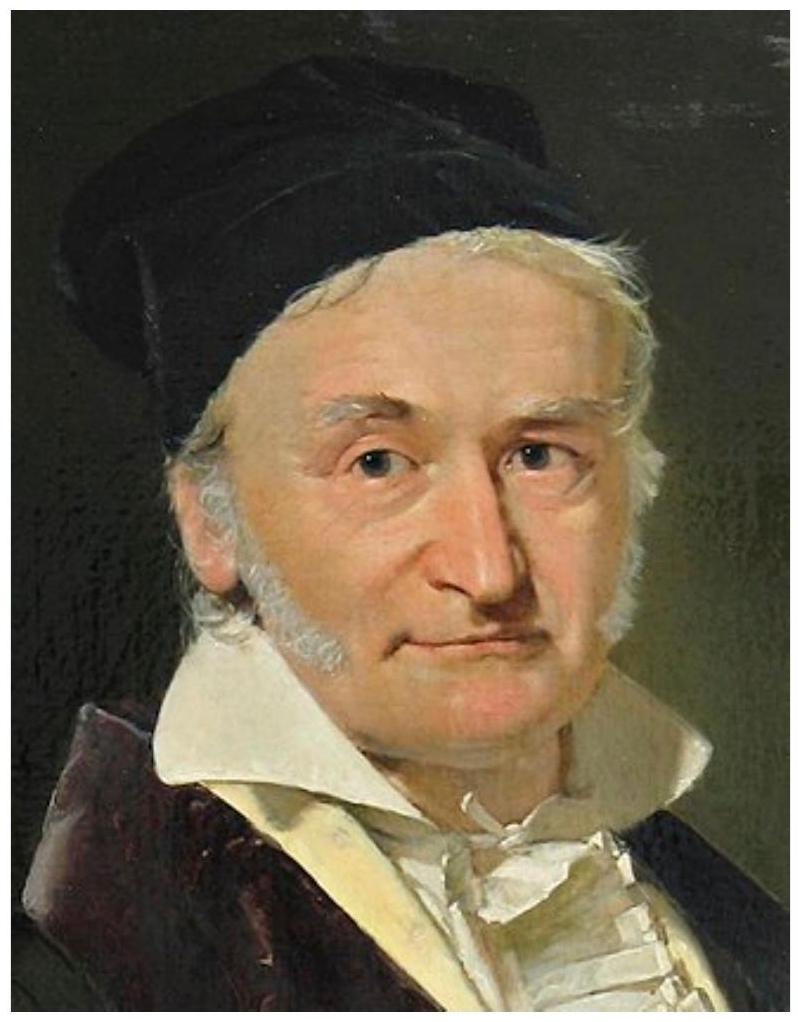
\includegraphics[max width=\textwidth, alt={}]{a51c6962-9810-4aca-832b-b8f33e898ec6-01_1022_798_377_218}
\end{center}

\section*{Carl Friedrich Gauss \\
 (1777-1855)}
\(1^{\text {er }}\) janvier 1801 : découverte de la planète naine Cérès par Piazzi à Palerme. Il la perd de vue

7 décembre 1801 : von Zachs retrouve Cérès dans la position exacte calculée par Gauss

\section*{APPROXIMATION par MOINDRES-CARRES}
Recherche d'un polynôme de degré au plus égal à \(n\) dont la distance à la solution est minimale.\\
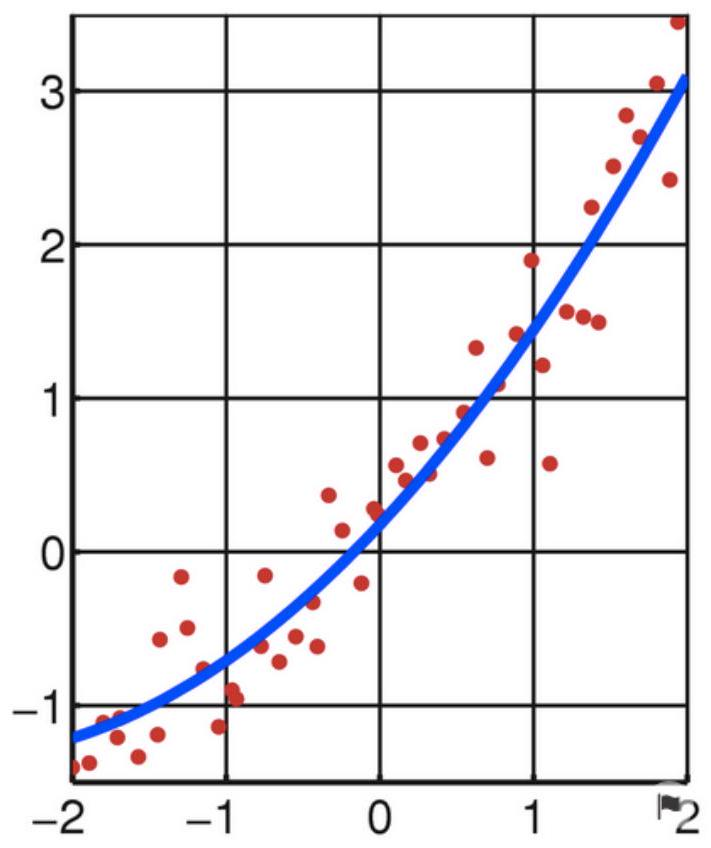
\includegraphics[max width=\textwidth, alt={}, center]{a51c6962-9810-4aca-832b-b8f33e898ec6-02_848_711_608_143}

La distance ar sens des moindres-carrés est la distance quadratipue qui s'écrit

\[
\delta^{2}=\int_{a}^{b} w(x)|P(x)-f(x)|^{2} d x
\]

Théorème.\\
Soit une fonction w(x.) intégrable strictement positive presque partout sur l'intervalle \([a, b]\) compact. Illexiste un unique poly notme \(P(x) \in \mathbb{P}_{n}\) tel que

\[
\forall Q \in \mathbb{P}_{n} \int_{a}^{b}|P(x)-f(x)|^{2} w(x) d x \leqslant
\]

Cepolynôme \(P(x)\) ast appelé approximation de of de degré au plus \(n\), au sehs des maindres-camés.

\section*{Attention :}
\begin{itemize}
  \item ordre du modèle (degré du polynôme)
  \item robustesse aux mesures aberrantes
\end{itemize}

\section*{MOTIVATION : MOINDRES CARRES}
Déterminer l'angle de tir de la trafe'ctiore parabolique issue de l'origine qui est estimée par la méthode des moindres carrés disposant des points:

\[
\begin{array}{lll}
P_{1} & x_{1}=1 & y_{1}=2 \\
P_{2} & x_{2}=2 & y_{2}=3 \\
P_{3} & x_{3}=3 & y_{3}=3,2 \\
P_{4} & x_{4}=4 & y_{4}=3,5 \\
P_{5} & x_{5}=5 & y_{5}=2,5
\end{array}
\]

Points de mesures entachés d'erreurs\\
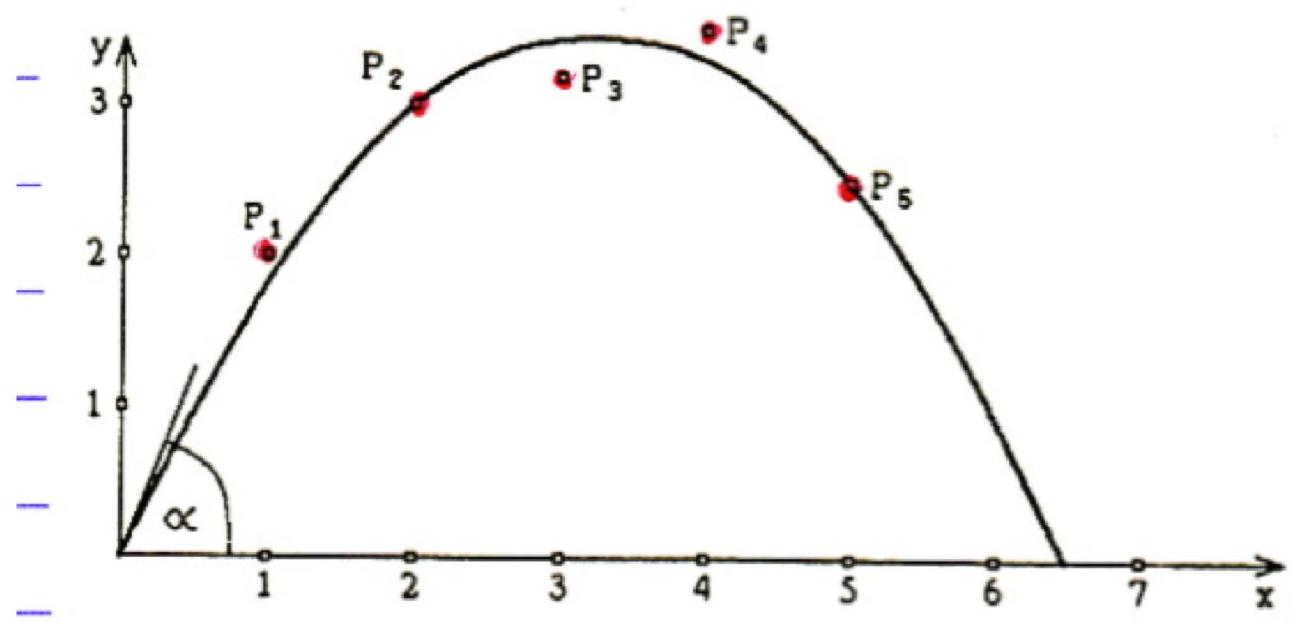
\includegraphics[max width=\textwidth, alt={}, center]{a51c6962-9810-4aca-832b-b8f33e898ec6-03_629_1304_1347_579}

\section*{MOTIVATION : MOINDRES CARRES}
On cherche une parabole qui minimise l'erreur (somme des distances carrées) entre la parabole (modèle physique) et les points. Meilleur ajustement\\
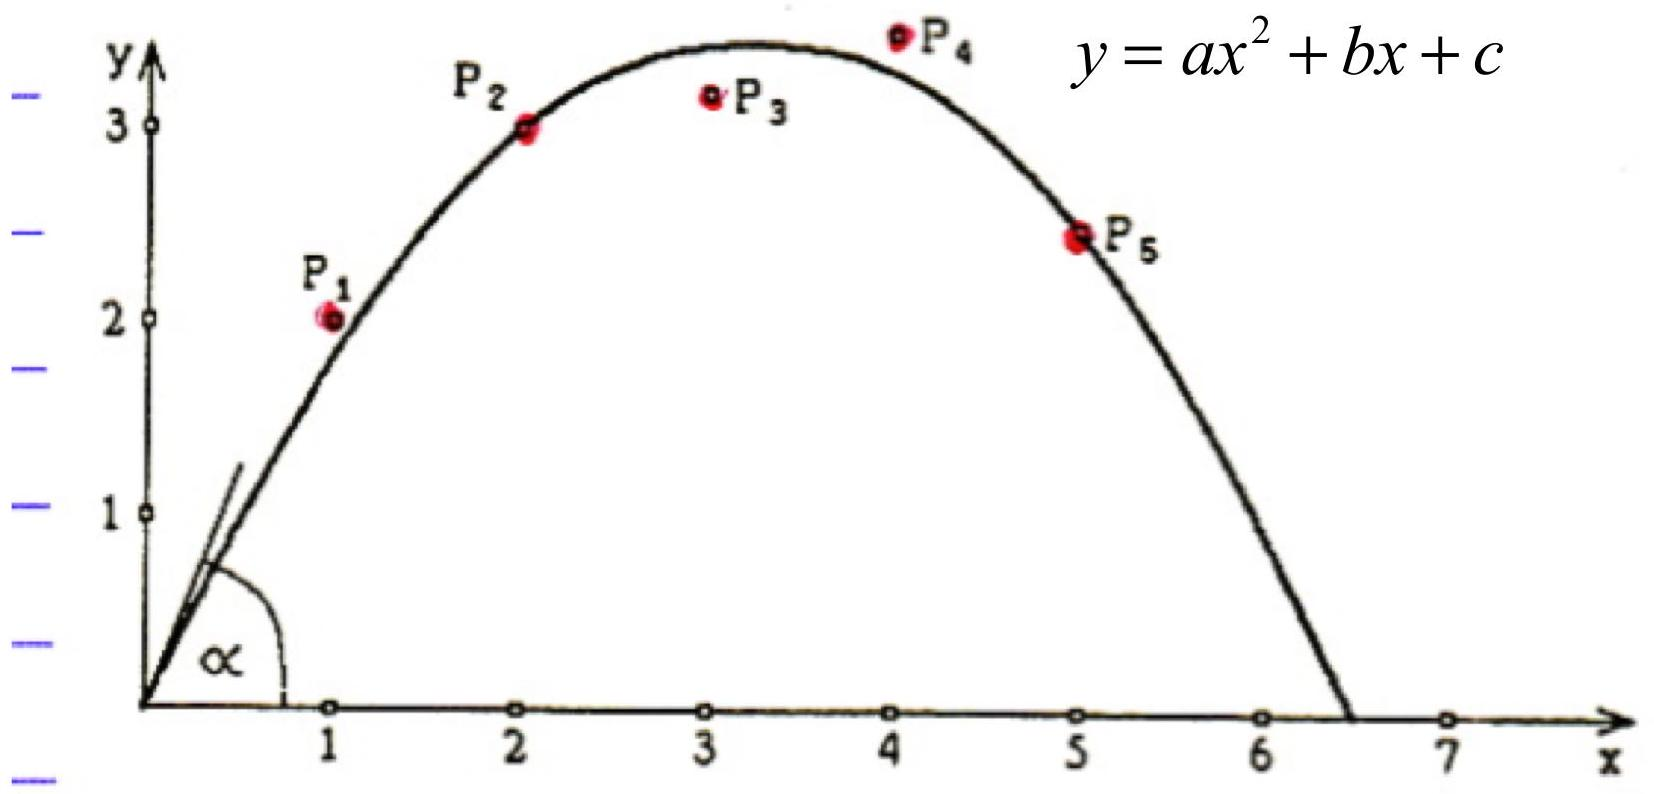
\includegraphics[max width=\textwidth, alt={}, center]{a51c6962-9810-4aca-832b-b8f33e898ec6-04_794_1654_699_161}\\
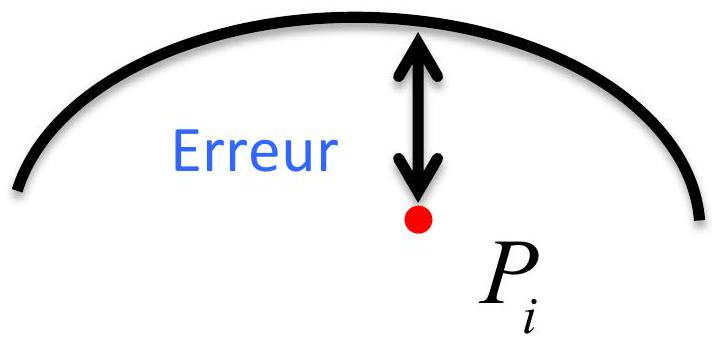
\includegraphics[max width=\textwidth, alt={}, center]{a51c6962-9810-4aca-832b-b8f33e898ec6-04_343_723_730_1932}

\[
y_{i}=a x_{i}^{2}+b x_{i}+\varepsilon_{i}
\]

Trouver (a,b) qui minimise

\[
\delta=\sum_{i=1}^{5}\left[a x_{i}^{2}+b x_{i}-y_{i}\right]^{2}
\]

\section*{MOTIVATION : MOINDRES CARRES}
Trouver \((a, b)\) qui minimise \(\quad \delta=\sum_{i=1}^{5}\left[a x_{i}^{2}+b x_{i}-y_{i}\right]^{2}\).\\
\(\delta\) minimale \(\Rightarrow \frac{\partial \delta}{\partial a}=0\) et \(\frac{\partial \delta}{\partial b}=0\)

\[
\left\{\begin{array}{l}
\sum_{i=1}^{5} \frac{\partial}{\partial a}\left[a x_{i}^{2}+b x_{i}-y_{i}\right]^{2}=0 \\
\sum_{i=1}^{5} \frac{\partial}{\partial b}\left[a x_{i}^{2}+b x_{i}-y_{i}\right]^{2}=0
\end{array}\right.
\]

\[
\left\{\begin{array}{l}
\sum_{i=1}^{\sum_{i=1}^{5} \frac{\partial}{\partial a}\left[a x_{i}^{2}+b x_{i}-y_{i}\right]^{2}=0} \\
\quad \begin{array}{l}
(1) \Rightarrow \sum_{i=1}^{5} 2\left[a x_{i}^{2}+b x_{i}-y_{i}\right]^{2}=0 \\
\left.a \sum_{i=1}^{5} x_{i}^{4}+b x_{i}-y_{i}\right] \sum_{i=1}^{2} x_{i}^{3}=0 \Rightarrow \sum_{i=1}^{5} y_{i} x_{i}^{2}
\end{array} \\
\quad(2) \Rightarrow \sum_{i=1}^{5} 2\left[a x_{i}^{2}+b x_{i}-y_{i}\right] x_{i}=0 \Rightarrow \\
\quad a \sum_{i=1}^{5} x_{i}^{3}+b \sum_{i=1}^{5} x_{i}^{2}=\sum_{i=1}^{5} x_{i} y_{i} .
\end{array}\right.
\]

\section*{MOTIVATION : MOINDRES CARRES}
\[
\left\{\begin{array}{l}
\frac{a \sum_{i=1}^{5} x_{i}^{4}+b \sum_{i=1}^{5} x_{i}^{3}=\sum_{i=1}^{5} y_{i} x_{i}^{2}}{a \sum_{i=1}^{5} x_{i}^{3}+b \sum_{i=1}^{5} x_{i}^{2}=\sum_{i=1}^{5} x_{i} y_{i}} \\
{\left[\begin{array}{ll}
\sum_{i=1}^{5} x_{i}^{4} & \sum_{i=1}^{5} x_{i}^{3} \\
\sum_{i=1}^{5} x_{i}^{3} & \sum_{i=1}^{5} x_{i}^{2}
\end{array}\right]\left[\begin{array}{l}
a \\
\sum_{i=1}^{5} x_{i}^{2} y_{i} \\
\sum_{i=1}^{5} x_{i} y_{i}
\end{array}\right]}
\end{array}\right.
\]

\section*{MOTIVATION : MOINDRES CARRES}
Il faut donc résoudre l'équation matricielle

\[
\begin{aligned}
{\left[\begin{array}{ll}
979 & 225 \\
225 & 55
\end{array}\right]\left[\begin{array}{l}
a \\
b
\end{array}\right] } & =\left[\begin{array}{c}
161,3 \\
44,1
\end{array}\right] \\
x & =5
\end{aligned}
\]

\(\operatorname{det} m=975 \times 55-225^{2}=53845-50625 \operatorname{det} M=3220 \neq 0\).

\[
\begin{gathered}
X=M^{-1} S \\
{\left[\begin{array}{l}
a \\
b
\end{array}\right]=\frac{1}{3220}\left[\begin{array}{cc}
55 & -225 \\
-225 & 979
\end{array}\right]\left[\begin{array}{c}
161.3 \\
44.1
\end{array}\right]}
\end{gathered}
\]

L'équation du mauvement s'écutalors:

\[
y=-0,3264 x^{2}+2,1371 x
\]

L'angle de tir a est défini par

\[
\begin{aligned}
& \operatorname{tg} \alpha=y^{\prime}(0) \Rightarrow \\
& \operatorname{tg} \alpha=b=8,1371
\end{aligned}
\]

D'aù \(\alpha=\) Arctg 2,1371 rad.

\[
\alpha=1,1331 \mathrm{rad} . \quad \alpha=64,92399^{\circ} .
\]

\begin{center}
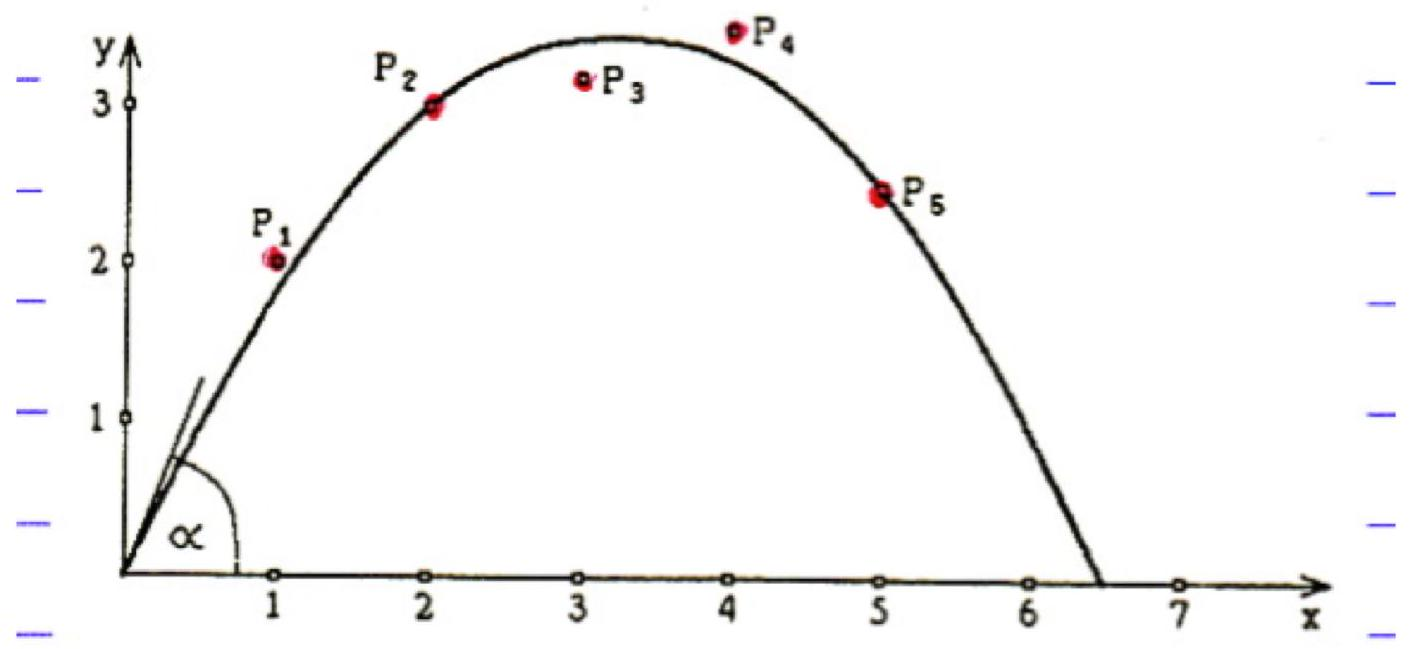
\includegraphics[max width=\textwidth, alt={}]{a51c6962-9810-4aca-832b-b8f33e898ec6-09_649_1414_1366_699}
\end{center}

\section*{MOINDRES CARRES : formalisme général}
Modèle des mesures

\[
y_{i}=a x_{i}^{2}+b x_{i}+\varepsilon_{i}
\]

\[
\underbrace{\left(\begin{array}{c}
y_{1} \\
\vdots \\
y_{n}
\end{array}\right)}_{Y(n, 1)}=\underbrace{\left(\begin{array}{cc}
x_{1}^{2} & x_{1} \\
\vdots & \vdots \\
x_{n}^{2} & x_{n}
\end{array}\right)}_{A(n, 2)} \underbrace{\binom{a}{b}}_{X(2,1)}+\varepsilon
\]

Trouver X qui minimise l'erreur quadratique

\[
\operatorname{Min}_{X}\|Y-A X\|^{2}=\operatorname{Min}_{X} C(X)
\]

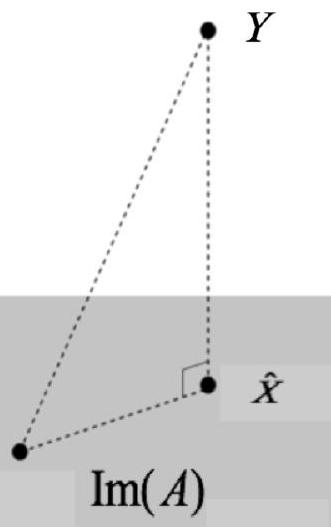
\includegraphics[max width=\textwidth, alt={}, center]{a51c6962-9810-4aca-832b-b8f33e898ec6-10_527_331_1068_2081}\\
\(\frac{\partial C}{\partial X}=-2 \underset{(2, n)}{A_{(n, 1)}^{T}} Y+2 A_{(2,1)}^{T} A X=0\)

\[
\hat{X}=\left(A^{T} A\right)^{-1} A^{T} Y
\]


\end{document}